\documentclass[11pt]{article}

\usepackage[utf8]{inputenc}
\usepackage[T1]{fontenc}
\usepackage[spanish,es-noshorthands,es-tabla]{babel}
\usepackage[margin=2.4cm]{geometry}
\usepackage{amsmath,amssymb}
\usepackage{graphicx}
\usepackage{float}
\usepackage{array}
\usepackage[hidelinks]{hyperref}

\graphicspath{{figuras/}}

\title{Curso Libre de Configuración 2: Análisis de Datos\\ Tarea 3: Introducción a series de tiempo}
\author{$<$ Jose Gregorio Coronel Colombo $>$ -- \texttt{jcoronel@unis.edu.gt}}
\date{Fecha de entrega: 25 de octubre 2026, 11:59PM}

\begin{document}
\maketitle

\section*{Uso de inteligencia artificial}

En este trabajo se usó inteligencia artificial como apoyo para escribir varios de los códigos
en Python a partir de las fórmulas y reglas del enunciado, para hacer algunas de las gráficas y
dar formato a las tablas, para resolver dudas de pandas y statsmodels, y para investigar temas
que no quedaban claros con los libros, como el sesgo del estimador OLS de $\phi$, por qué el
modelo de aerolínea extrapola una pendiente y cómo se calcula el AUC con rangos. También se usó
para ordenar la redacción del documento a partir de los resultados. La semilla, qué líneas
cuentan como venta, el orden de las reglas de limpieza y las derivaciones del inciso 0.1 se
hicieron sin IA, y los números del texto se revisaron contra la salida de los scripts. Al inicio
de cada archivo \texttt{.py} se indica para qué se usó la IA en ese archivo.

\section*{Reproducibilidad y semillas}

Todo sale del archivo original \texttt{datos/Online Retail.xlsx}, que va incluido en el
repositorio tal como se descarga de UCI. Desde la carpeta \texttt{codigo/}, los cuatro scripts

\begin{center}\ttfamily
python3 generar\_resultados\_procesos\_simulados.py\\
python3 generar\_resultados\_limpieza\_calendario.py\\
python3 generar\_resultados\_series\_pronostico.py\\
python3 generar\_resultados\_rfm.py
\end{center}

\noindent
vuelven a producir todas las figuras y todas las tablas de este informe. Cada script guarda sus
figuras en \texttt{figuras/} e imprime las tablas ya escritas en \LaTeX{}, que son las que
aparecen incrustadas en este documento. La función \texttt{limpiar} está sola en
\texttt{limpieza\_datos.py}, como pide el enunciado.

La semilla base es la misma de la Tarea 2, 552003. En la Parte 0 cada escenario usa un múltiplo
distinto, para que ningún escenario comparta números aleatorios con otro, y las diez
repeticiones de la validación cruzada de 5.2 usan los diez primeros múltiplos. La única semilla
que no sale de 552003 es la del desempate de 6.2, que el enunciado fija en 2026.

\begin{table}[H]
\centering
\caption{Semillas de cada experimento.}\label{tab:semillas}
\begin{tabular}{|l|l|}
\hline
Experimento & Semilla usada \\
\hline
AR(1) con $\phi = 0,\ 0.5,\ 0.9,\ 1$ (0.2) & $552003\cdot 1$, $\cdot 2$, $\cdot 3$, $\cdot 4$ \\
Tendencia lineal (0.4 a) & $552003\cdot 5$ \\
Patrón semanal (0.4 b) & $552003\cdot 6$ \\
Validación cruzada aleatoria (5.2 a) & $552003\cdot k$, $k = 1,\dots,10$ \\
Desempate de los puntajes RFM (6.2) & 2026 (fijada por el enunciado) \\
\hline
\end{tabular}
\end{table}

\section*{Parte 0: procesos simulados}

\subsection*{Inciso 0.1: momentos del AR(1) y de la caminata aleatoria}

Sea $Y_t = c + \phi Y_{t-1} + \varepsilon_t$ con $\varepsilon_t \overset{iid}{\sim} N(0,\sigma^2)$,
$|\phi|<1$ y el proceso estacionario, de modo que $E[Y_t]=E[Y_{t-1}]=\mu$ y
$\operatorname{Var}(Y_t)=\operatorname{Var}(Y_{t-1})=\gamma_0$.

Media. Tomando esperanza en los dos lados y usando $E[\varepsilon_t]=0$,
\[
\mu = c + \phi\mu \quad\Longrightarrow\quad \mu(1-\phi)=c \quad\Longrightarrow\quad
E[Y_t]=\frac{c}{1-\phi}.
\]
La división es válida porque $\phi\neq 1$.

Varianza. La constante no aporta varianza. $Y_{t-1}$ depende solo de
$\varepsilon_{t-1},\varepsilon_{t-2},\dots$, así que es independiente de $\varepsilon_t$ y la
covarianza cruzada es cero:
\[
\gamma_0 = \operatorname{Var}(\phi Y_{t-1}+\varepsilon_t) = \phi^2\gamma_0 + \sigma^2
\quad\Longrightarrow\quad \operatorname{Var}(Y_t)=\frac{\sigma^2}{1-\phi^2},
\]
que es positiva porque $\phi^2<1$.

Autocorrelación. Para $k\ge 1$, $\varepsilon_t$ también es independiente de
$Y_{t-k}$, así que
\[
\gamma_k = \operatorname{Cov}(c+\phi Y_{t-1}+\varepsilon_t,\;Y_{t-k})
= \phi\operatorname{Cov}(Y_{t-1},Y_{t-k}) = \phi\,\gamma_{k-1}.
\]
Aplicando la recursión $k$ veces, $\gamma_k=\phi^k\gamma_0$, y dividiendo entre $\gamma_0$,
$\rho_k=\phi^k$.

Caminata aleatoria. Con $\phi=1$, $c=0$ y $Y_0=0$, desenrollando la recursión,
$Y_t = \varepsilon_1+\varepsilon_2+\dots+\varepsilon_t$. Como los $\varepsilon_i$ son
independientes, las varianzas se suman:
\[
\operatorname{Var}(Y_t)=\sum_{i=1}^{t}\operatorname{Var}(\varepsilon_i)=t\sigma^2 .
\]
La varianza crece con $t$, y la estacionariedad débil exige que no dependa del momento en que
se observa. También la covarianza depende de $t$, porque
$\operatorname{Cov}(Y_t,Y_{t-k})=(t-k)\sigma^2$. La fórmula de la varianza estacionaria lo
anticipa, ya que con $\phi=1$ queda $\sigma^2/0$ y no hay ninguna varianza fija a la que el
proceso pueda llegar.

\subsection*{Inciso 0.2: simulación}

La función \texttt{simular\_ar1} arranca en $Y_0=0$, avanza 500 pasos y conserva los últimos
300, con $c=0$ y $\sigma=1$. Para $\phi<1$ el calentamiento sirve porque el efecto del valor
inicial se apaga como $\phi^{200}$, que con $\phi=0.9$ ya vale $7\times10^{-10}$. Con $\phi=1$
no se apaga nunca, pero tampoco importa para $r_k$. Lo que se conserva es
$Y_{200}+(\varepsilon_{201}+\dots+\varepsilon_t)$, es decir, una caminata que arranca en el valor
$Y_{200}$ en vez de en cero. Sumarle una constante a toda la serie también se la suma a
$\bar y$, y $r_k$ solo usa las desviaciones $y_t-\bar y$, que no cambian. Por eso $r_k$ es el
mismo arranque donde arranque.

\begin{figure}[H]
\centering
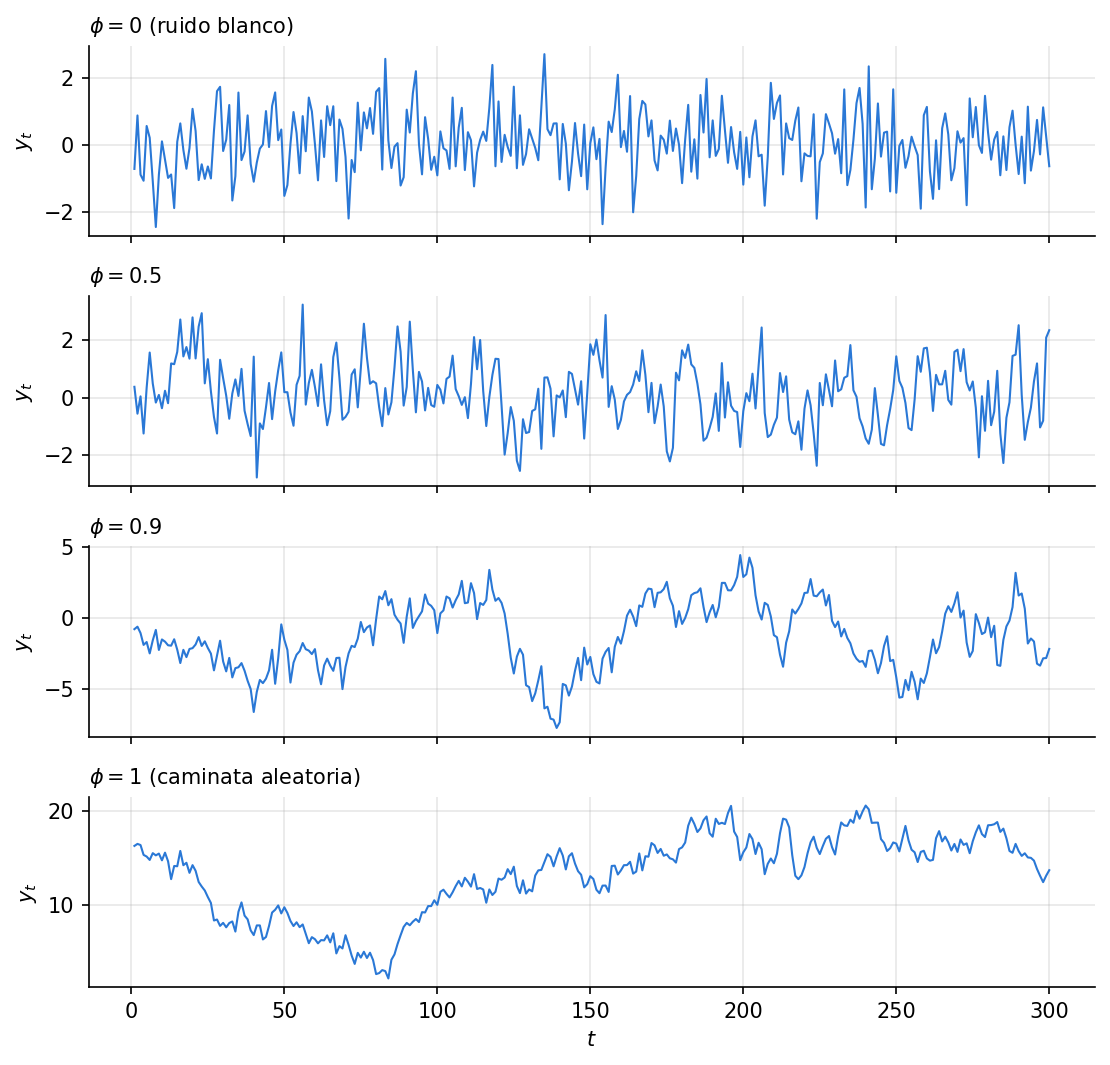
\includegraphics[width=0.9\textwidth]{realizaciones_ar1.png}
\caption{Una realización de cada AR(1). Con $\phi=0$ la serie no tiene ninguna inercia. Con
$\phi=0.5$ se ven rachas cortas, con $\phi=0.9$ rachas largas que siempre vuelven a cero, y la
caminata aleatoria se aleja sin volver a ninguna media.}
\label{fig:realizaciones-ar1}
\end{figure}

La tabla~\ref{tab:ar1} resume las 5\,000 réplicas de cada escenario. Entre paréntesis va el
error estándar del promedio, $s/\sqrt{5000}$, y para la tasa de rechazo
$\sqrt{\hat p(1-\hat p)/5000}$, porque una tasa es el promedio de una indicadora.

\begin{table}[H]
\centering
\caption{Resultados de 5\,000 réplicas de $n=300$ por escenario. Entre paréntesis, el error
estándar de cada promedio.}\label{tab:ar1}
\small
\begin{tabular}{|c|c|c|c|c|c|}
\hline
$\phi$ & $\bar r_1$ & $\bar r_5$ & $\phi^5$ & Tasa de rechazo con $r_1$ & $\bar{\hat\phi}_{\text{OLS}}$ \\
\hline
0 & -0.0015 (0.0008) & -0.0038 (0.0008) & 0.0000 & 0.0522 (0.0031) & -0.0015 (0.0008) \\
0.5 & 0.4905 (0.0007) & 0.0211 (0.0010) & 0.0312 & 1.0000 (0.0000) & 0.4922 (0.0007) \\
0.9 & 0.8837 (0.0004) & 0.5333 (0.0014) & 0.5905 & 1.0000 (0.0000) & 0.8870 (0.0004) \\
1 & 0.9752 (0.0002) & 0.8810 (0.0009) & 1.0000 & 1.0000 (0.0000) & 0.9817 (0.0002) \\
\hline
\end{tabular}
\end{table}

\subsection*{Inciso 0.3: lo que dice la tabla}

Ruido blanco. Con $\phi=0$ la prueba rechaza en el 5.22\,\% de las réplicas, a menos
de un error estándar del 5\,\% nominal. Es lo que se esperaba, porque bajo ruido blanco
$r_1\approx N(0,1/n)$ y la banda $\pm1.96/\sqrt n$ está construida para dejar fuera justo el
5\,\% de esa normal. Cada rechazo aquí es un error tipo I, como el rechazo de Blum Blum Shub en
la Tarea 2. Con $\phi=0.5$ en adelante la prueba rechaza siempre, porque $r_1$ queda a más de
cuatro bandas de cero.

Caminata aleatoria. La teoría $\rho_5=\phi^5$ dice 1 y la simulación da 0.881. La
fórmula $\rho_k=\phi^k$ se derivó suponiendo estacionariedad, y la caminata no lo es, así que
no hay ningún $\rho_k$ que estimar. Lo que mide $r_k$ en una caminata es qué tanto se parece
la trayectoria a sí misma corrida $k$ pasos, y como $\bar y$ es la media de una sola
trayectoria que deambula, $r_k$ sale grande pero lejos de 1 y bajando despacio con $k$ (figura
\ref{fig:acf-simulados}). La firma de una serie no estacionaria es justamente esa ACF que no
cae.

Sesgo del OLS. El estimado de $\phi$ queda siempre por debajo del verdadero, y el
sesgo crece con $\phi$: $-0.0015$, $-0.0078$, $-0.0130$ y $-0.0183$. Para $\phi=0.5$ y $0.9$
cuadra con la aproximación clásica $-(1+3\phi)/n$, que da $-0.0083$ y $-0.0123$. Para la
caminata el sesgo es más grande que lo que predice esa fórmula, porque ahí la distribución del
estimador deja de ser normal (es la distribución de Dickey--Fuller). El sesgo aparece porque el
regresor $y_{t-1}$ no es independiente de los errores pasados y porque se estima la media con
la misma muestra. Aun así el estimador es consistente, ya que el sesgo es de orden $1/n$ y
desaparece al crecer la muestra. Con 300 datos es pequeño frente al error de una réplica
suelta, pero para $\phi\ge0.5$ está a más de diez errores estándar de cero, así que es un sesgo
y no ruido. El
promedio de $r_1$ subestima todavía más que el OLS (0.8837 contra 0.8870 con $\phi=0.9$).

\subsection*{Inciso 0.4: las dos razones para reprobar}

\begin{figure}[H]
\centering
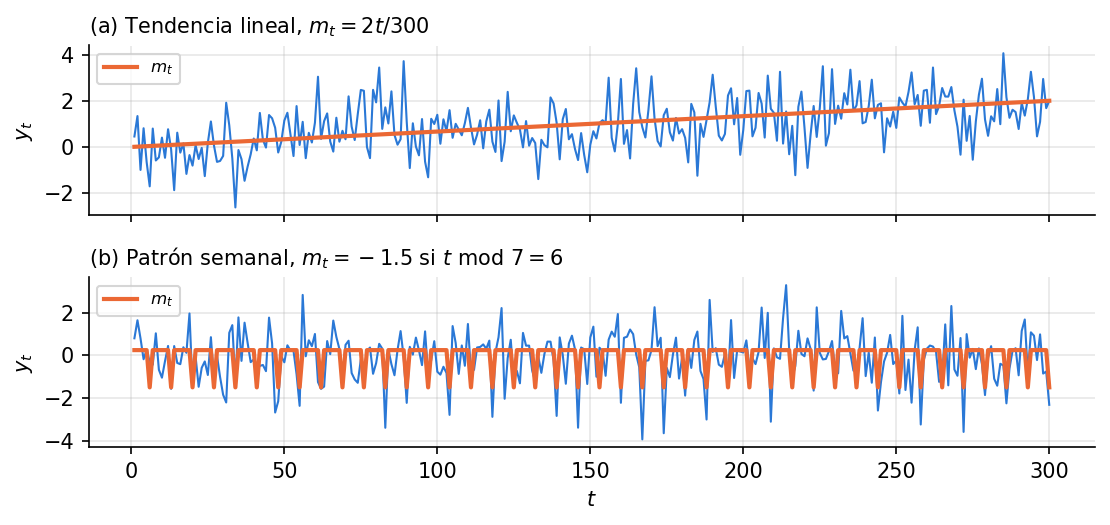
\includegraphics[width=0.9\textwidth]{realizaciones_sin_memoria.png}
\caption{Una realización de cada proceso sin memoria. En naranja la media $m_t$, que es lo único
que cambia con el tiempo. El ruido alrededor de $m_t$ es independiente día a día.}
\label{fig:sin-memoria}
\end{figure}

\begin{table}[H]
\centering
\caption{Procesos sin memoria con media que cambia en el tiempo, 5\,000 réplicas cada uno. El
ruido blanco se repite como referencia.}\label{tab:sin-memoria}
\resizebox{\textwidth}{!}{
\begin{tabular}{|l|c|c|c|c|c|}
\hline
Proceso & $\bar r_1$ & $\bar r_5$ & $\bar r_7$ & Tasa de rechazo con $r_1$ & $\bar{\hat\phi}_{\text{OLS}}$ \\
\hline
Ruido blanco ($\phi=0$) & -0.0015 (0.0008) & -0.0038 (0.0008) & -0.0036 (0.0008) & 0.0522 (0.0031) & -0.0015 (0.0008) \\
(a) Tendencia lineal & 0.2455 (0.0008) & 0.2359 (0.0008) & 0.2304 (0.0008) & 0.9850 (0.0017) & 0.2467 (0.0008) \\
(b) Patrón semanal & -0.0467 (0.0007) & -0.0481 (0.0007) & 0.2640 (0.0008) & 0.1054 (0.0043) & -0.0470 (0.0007) \\
\hline
\end{tabular}}
\end{table}

La tendencia lineal reprueba la prueba de retardo 1 en el 98.5\,\% de las réplicas aunque no
tiene memoria. El mecanismo es el de la razón (2) del enunciado: $\bar y$ queda a media altura,
los días del principio están todos por debajo y los del final todos por encima, y dos días
vecinos casi siempre caen del mismo lado. Por eso $r_1$, $r_5$ y $r_7$ salen casi iguales
(0.25, 0.24, 0.23). Una memoria verdadera decaería como $\phi^k$. Aquí no decae porque no hay
memoria, sino un nivel que se mueve. El OLS cae en la misma trampa y reporta un
$\hat\phi=0.247$ que no existe.

El patrón semanal hace lo contrario: tiene una estructura muy marcada y pasa la prueba en casi
nueve de cada diez réplicas. Su $r_1$ es $-0.047$, y se puede calcular a mano. Las desviaciones
de $m_t$ respecto a su media (que es cero) son $0.25$ seis días y $-1.5$ uno, así que de los
siete productos de vecinos de cada semana cinco valen $0.0625$ y dos valen $-0.375$, en total
$-0.4375$ por semana. Dividido entre la varianza total por día, $0.375+1$, da
$-0.4375/(7\cdot1.375)=-0.045$. Es un número tan pequeño que queda dentro de la banda. Toda la
estructura está en el rezago 7, donde $r_7=0.264$ (a mano, $0.375/1.375=0.273$). El rechazo sube
de 5\,\% a 10.5\,\% solo porque $r_1$ está corrido un poco hacia abajo.

Ese segundo caso es RANDU en la Tarea 2. RANDU pasó la prueba de autocorrelación de retardo 1
con un $p$-valor cómodo y, sin embargo, cada número está determinado por los dos anteriores
($x_{k+2}=6x_{k+1}-9x_k$), y por eso todas las ternas caen en 15 planos. En los dos casos la
estructura vive en un lugar que la prueba no mira (el rezago 7 aquí, las ternas allá). Una
prueba solo ve dependencia en los rezagos que examina.

\begin{figure}[H]
\centering
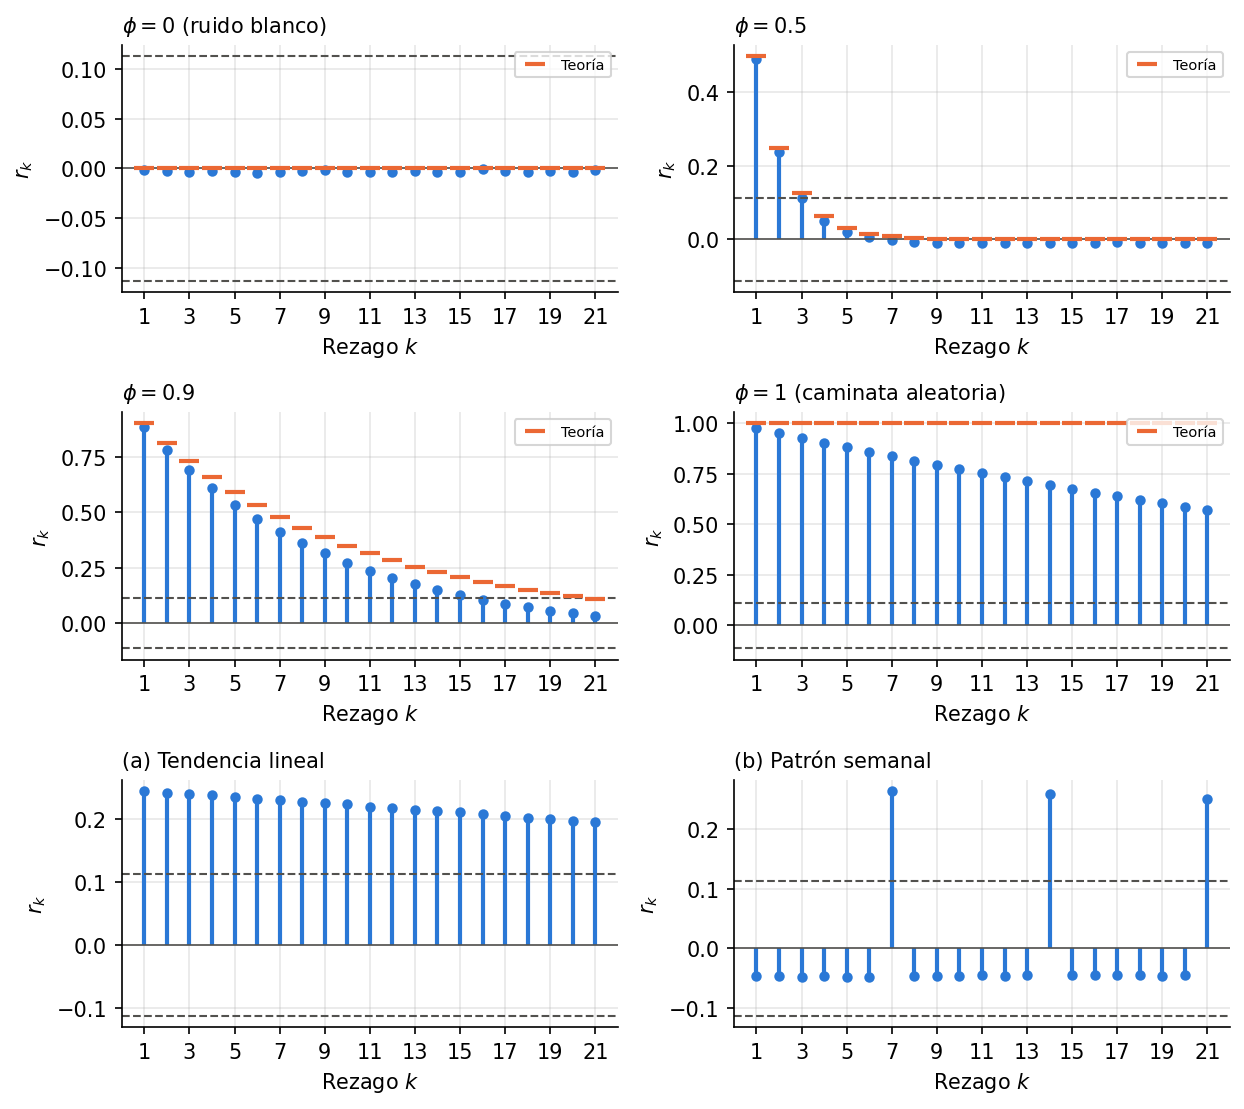
\includegraphics[width=\textwidth]{acf_promedio_procesos_simulados.png}
\caption{ACF promedio de las 5\,000 réplicas de cada proceso, con las bandas $\pm1.96/\sqrt{300}$.
En naranja, la teoría $\phi^k$ para los AR(1). La tendencia produce una ACF alta y casi plana
sin tener memoria, y el patrón semanal produce picos en 7, 14 y 21 con $r_1$ casi nulo.}
\label{fig:acf-simulados}
\end{figure}

\subsection*{Inciso 0.5: la prueba que sí ve}

La Ljung--Box propia (\texttt{autocorrelacion.ljung\_box}) se comparó contra
\texttt{acorr\_ljungbox} de statsmodels en las 15\,000 series de la tabla~\ref{tab:ljung-box}. La
diferencia máxima en $Q(10)$ fue de $4\times10^{-13}$, que es redondeo de punto flotante. Se
reportan los dos valores de $m$ que discute el enunciado: $m=10$ de FPP2 y $m\approx\log 300=5.7$,
que se redondea a 6, de Tsay.

\begin{table}[H]
\centering
\caption{Tasa de rechazo al 5\,\% de cada prueba, 5\,000 réplicas por proceso.}\label{tab:ljung-box}
\begin{tabular}{|l|c|c|c|}
\hline
Proceso & Prueba con $r_1$ & Ljung--Box ($m=6$) & Ljung--Box ($m=10$) \\
\hline
Ruido blanco ($\phi=0$) & 0.0522 (0.0031) & 0.0508 (0.0031) & 0.0508 (0.0031) \\
(a) Tendencia lineal & 0.9850 (0.0017) & 1.0000 (0.0000) & 1.0000 (0.0000) \\
(b) Patrón semanal & 0.1054 (0.0043) & 0.2004 (0.0057) & 0.9546 (0.0029) \\
\hline
\end{tabular}
\end{table}

Con ruido blanco la Ljung--Box rechaza el 5.08\,\%, igual que el nivel nominal, así que juntar
rezagos no infla el error tipo I. La tendencia la reprueban todas. El cambio está en el patrón
semanal: con $m=10$ el rechazo pasa del 10.5\,\% de la prueba de retardo 1 al 95.5\,\%, porque
$Q(10)$ suma $r_7^2$ y $r_7$ es grande. Con $m=6$ se queda en 20\,\%, porque el rezago 7 queda
fuera de la suma, y lo poco que sube viene de que los $r_1,\dots,r_6$ están todos corridos a
$-0.047$. La comparación entre los dos libros se decide sola en este caso. La regla de FPP2
($m=10$ sin estacionalidad, $m=2s$ con ella) cubre el periodo, y $\log n$ no. Una portmanteau
solo ve la estacionalidad si $m$ llega hasta el periodo.

\section*{Parte 1: limpieza}

\subsection*{Inciso 1.1: los datos crudos}

El archivo tiene 541\,909 filas, 25\,900 facturas, 4\,070 productos y 4\,372 clientes. El 24.93\,\%
de las filas (135\,080) no tiene \texttt{CustomerID}.

Las tres columnas se leen como texto porque son etiquetas y no cantidades. Si se deja que pandas
adivine el tipo, \texttt{InvoiceNo} queda como una columna mezclada de 532\,618 enteros y 9\,291
cadenas. Con eso \texttt{.str.startswith("C")} devuelve faltantes en todas las facturas
normales y la regla de cancelaciones se rompe. \texttt{StockCode} queda con 487\,036 enteros y
54\,873 cadenas, de modo que \texttt{85123} y \texttt{85123A} quedan de distinto tipo y no se
pueden comparar con una sola expresión regular. \texttt{CustomerID} queda como
\texttt{float64}, porque los faltantes obligan a pandas a usar flotantes, y el cliente 17850
aparece como \texttt{17850.0}. Ninguna operación aritmética sobre estas columnas tiene sentido.

\subsection*{Inciso 1.2: qué es una venta}

El criterio que se adoptó es que cuenta como venta todo lo que es mercancía y todo lo que ajusta
el precio de mercancía vendida. Lo que es un cobro distinto (envío, comisiones) o un movimiento
de inventario se va.

(a) Duplicados exactos: se van. Hay 5\,268 filas idénticas a otra en las ocho
columnas, incluida la hora al minuto. Una misma factura no repite el mismo producto en dos
líneas idénticas (lo normal es sumar la cantidad), así que se tratan como registros dobles del
sistema. Representan \textsterling{}21\,741 netas.

(b) Facturas que no empiezan con dígito. Hay dos prefijos. Las 9\,288 filas con C
(3\,836 facturas) son cancelaciones y se quedan: todas traen ya la cantidad negativa,
así que no hace falta transformarlas, y al sumar restan el día en que ocurren, como pide el
enunciado. Las 3 filas con A (\texttt{A563185} a \texttt{A563187}) son asientos contables
``Adjust bad debt'' por \textsterling{}11\,062.06, sin cliente ni producto. Se van, porque una
deuda incobrable no es una venta.

(c) Códigos que no son productos. La tabla~\ref{tab:codigos} lista los códigos que
no empiezan con cinco dígitos. No todos son iguales. \texttt{DCGS*}, los vales de regalo
\texttt{gift\_0001\_*} y \texttt{PADS} son productos con código especial y se quedan. Los
envíos (\texttt{POST}, \texttt{DOT}, \texttt{C2}) son un cobro aparte de la mercancía (casi todo
\texttt{DOT} va sin cliente), y las comisiones de Amazon, del banco y de CRUK son costos de la
tienda, no ventas, así que todos se van. Las muestras \texttt{S} y la deuda \texttt{B} también se
van. \texttt{M} (ajuste manual) y \texttt{D} (descuento) se quedan porque corrigen el precio de
ventas que sí ocurrieron. El caso que lo decide está en el inciso 1.4: sin \texttt{M} quedaría
contada una venta de \textsterling{}38\,970 que la tienda anuló con un ajuste manual tres minutos después.

\begin{table}[H]
\centering
\caption{Códigos de \texttt{StockCode} que no empiezan con cinco dígitos, en los datos crudos.}\label{tab:codigos}
\small
\begin{tabular}{|l|l|r|r|l|}
\hline
Código & Descripción & Filas & Monto (\textsterling{}) & Decisión \\
\hline
\texttt{POST} & POSTAGE & 1\,256 & 66\,230.64 & Se va \\
\texttt{DOT} & DOTCOM POSTAGE & 710 & 206\,245.48 & Se va \\
\texttt{M} & Manual & 571 & -68\,674.19 & Se queda \\
\texttt{C2} & CARRIAGE & 144 & 6\,986.00 & Se va \\
\texttt{D} & Discount & 77 & -5\,696.22 & Se queda \\
\texttt{S} & SAMPLES & 63 & -3\,049.39 & Se va \\
\texttt{BANK CHARGES} & Bank Charges & 37 & -7\,175.64 & Se va \\
\texttt{AMAZONFEE} & AMAZON FEE & 34 & -221\,520.50 & Se va \\
\texttt{CRUK} & CRUK Commission & 16 & -7\,933.43 & Se va \\
\texttt{B} & Adjust bad debt & 3 & -11\,062.06 & Se va \\
\texttt{m} & Manual & 1 & 2.55 & Se queda \\
\texttt{DCGS*} & productos con código especial & 45 & 398.45 & Se queda \\
\texttt{gift\_0001\_*} & productos con código especial & 34 & 685.81 & Se queda \\
\texttt{PADS} & productos con código especial & 4 & 0.00 & Se queda \\
\hline
\end{tabular}
\end{table}

(d) Precio cero o negativo: se van. Hay 2\,515 filas con precio cero y 2 con precio
negativo. Las dos negativas son asientos A del inciso (b). Las de precio cero son en un 98\,\%
filas sin cliente (casi todas los ajustes de inventario del inciso e), y las que tienen
cliente son regalos o muestras sin cobro. No mueven dinero, así que quitarlas no cambia la venta
diaria, pero dejarlas inflaría el conteo de facturas, y con él la frecuencia de la Parte 6.

(e) Cantidad negativa sin ser cancelación: se van. Son 1\,336 filas, todas con precio
cero y sin cliente. Su descripción es una nota de bodega: vacía en 862, y en el resto
``check'', ``damages'', ``damaged'', ``?'', ``thrown away'', ``sold as set on dotcom''. Son ajustes
de inventario (mercancía dañada, perdida o recontada) y no una venta devuelta, así que se van.
Tampoco mueven dinero.

(f) Filas sin \texttt{CustomerID}: se quedan en la serie. En los datos limpios son
131\,687 filas (24.8\,\%) y \textsterling{}1\,496\,241. Son ventas que ocurrieron aunque no se sepa a quién,
así que la venta diaria las necesita. En la Parte 6 la pregunta es quién compró, y ahí no sirven,
así que se quitan solo en esa parte.

\subsection*{Inciso 1.3: bitácora de limpieza}

\begin{table}[H]
\centering
\caption{Bitácora de limpieza. Las reglas se aplican en el orden de la primera columna y cada
una cuenta solo las filas que siguen vivas. El monto absoluto suma $|$Quantity $\times$
UnitPrice$|$ y muestra cuánto dinero movían esas filas aunque se compensen entre sí.}\label{tab:bitacora}
\small
\begin{tabular}{|c|l|r|r|r|}
\hline
Orden & Regla & Filas eliminadas & Neto (\textsterling{}) & Absoluto (\textsterling{}) \\
\hline
1 & Duplicados exactos & 5\,268 & 21\,740.98 & 27\,406.50 \\
2 & Facturas con prefijo A (ajuste de deuda) & 3 & -11\,062.06 & 33\,186.18 \\
3 & Cantidad negativa sin ser cancelación & 1\,336 & 0.00 & 0.00 \\
4 & Códigos que no son mercancía & 2\,259 & 39\,792.90 & 570\,988.68 \\
5 & Precio igual a cero o negativo & 1\,166 & 0.00 & 0.00 \\
\hline
-- & Sin \texttt{CustomerID} (se quedan en la serie) & 131\,687 & 1\,496\,240.86 & 1\,573\,779.90 \\
\hline
& Datos crudos & 541\,909 & 9\,747\,747.93 & \\
& Datos limpios & 531\,877 & 9\,697\,276.11 & \\
\hline
\end{tabular}
\end{table}

El orden cambia los conteos. La regla 5 solo quita 1\,166 filas porque 1\,351 de las que
cumplen esa condición ya se habían ido: las 1\,336 de cantidad negativa (todas con precio cero),
las dos de precio negativo y 13 que ya habían caído como duplicados o códigos que no son
mercancía. Si fuera primera, quitaría 2\,517. El monto neto de la regla 4 es pequeño (\textsterling{}39\,793) pero su monto absoluto
es de \textsterling{}571\,000, porque mezcla \textsterling{}279\,000 de envíos con \textsterling{}221\,000 de comisiones de Amazon que se
compensan. Esas líneas mueven mucho dinero aunque su suma neta sea pequeña. La limpieza
completa quita 10\,032 filas y cambia la venta total en solo 0.5\,\%, pero lo que quita está
concentrado en días puntuales (la mitad de las comisiones de Amazon pasan de \textsterling{}5\,900 y la más
grande es de \textsterling{}17\,836) y movería esos días bastante.

\subsection*{Inciso 1.4: las seis líneas más grandes}

\begin{table}[H]
\centering
\caption{Las seis líneas con mayor $|$Quantity $\times$ UnitPrice$|$ en los datos crudos.}\label{tab:lineas-grandes}
\resizebox{\textwidth}{!}{
\begin{tabular}{|l|l|l|r|r|l|l|r|}
\hline
Factura & Código & Descripción & Cantidad & Precio & Fecha & Cliente & Monto (\textsterling{}) \\
\hline
581483 & \texttt{23843} & PAPER CRAFT , LITTLE BIRDIE & 80\,995 & 2.08 & 09/12/2011 09:15 & 16446 & 168\,469.60 \\
C581484 & \texttt{23843} & PAPER CRAFT , LITTLE BIRDIE & -80\,995 & 2.08 & 09/12/2011 09:27 & 16446 & -168\,469.60 \\
541431 & \texttt{23166} & MEDIUM CERAMIC TOP STORAGE JAR & 74\,215 & 1.04 & 18/01/2011 10:01 & 12346 & 77\,183.60 \\
C541433 & \texttt{23166} & MEDIUM CERAMIC TOP STORAGE JAR & -74\,215 & 1.04 & 18/01/2011 10:17 & 12346 & -77\,183.60 \\
556444 & \texttt{22502} & PICNIC BASKET WICKER 60 PIECES & 60 & 649.50 & 10/06/2011 15:28 & 15098 & 38\,970.00 \\
C556445 & \texttt{M} & Manual & -1 & 38970.00 & 10/06/2011 15:31 & 15098 & -38\,970.00 \\
\hline
\end{tabular}}
\end{table}

Las seis líneas son tres pedidos y sus tres anulaciones, y en los tres casos la anulación llegó
el mismo día y en minutos.

\begin{itemize}
\item 80\,995 PAPER CRAFT, LITTLE BIRDIE (\textsterling{}168\,470). El cliente 16446 solo había hecho
una compra de \textsterling{}2.90 en mayo. A las 9:15 del 9 de diciembre aparece un pedido de casi 81\,000
unidades, y doce minutos después la cancelación exacta. Es un error de captura de la cantidad.
\item 74\,215 MEDIUM CERAMIC TOP STORAGE JAR (\textsterling{}77\,184). El cliente 12346 tiene en todo el
año esas dos líneas y nada más: el pedido y su cancelación dieciséis minutos después. Es el
mismo tipo de error.
\item 60 PICNIC BASKET WICKER 60 PIECES (\textsterling{}38\,970). El cliente 15098 compró a las 15:22
sesenta canastas pequeñas a \textsterling{}4.95. A las 15:28 se registró el paquete de 60 piezas con cantidad
60 y precio \textsterling{}649.50, que es el precio del paquete completo, así que se cobraron 60 paquetes. A las
15:31 un ajuste manual \texttt{M} devolvió exactamente \textsterling{}38\,970. A las 15:33 se volvió a registrar
el paquete con cantidad 1, y a las 15:39 se cancelaron las sesenta canastas sueltas. El neto del
cliente ese día es \textsterling{}649.50, que es lo que de verdad compró.
\end{itemize}

La limpieza no las resuelve, y no debería. Las seis sobreviven, porque son productos o ajustes
\texttt{M} y las cancelaciones se quedan a propósito. Una regla que borrara cantidades
``demasiado grandes'' quitaría el pedido y dejaría su cancelación, y eso inventaría un día con
\textsterling{}168\,000 negativos. Lo que sí las resuelve es netear por día: cada par cae el mismo día y suma
cero, y en el caso del picnic el día queda con los \textsterling{}649.50 correctos. La primera además cae en el
9 de diciembre, que se descarta en el inciso 2.4. Por cliente el neteo resuelve el monto pero no
la frecuencia. El cliente 12346 llega a la Parte 6 con $F=1$ y $M=0$.

\subsection*{Inciso 1.5: la función \texttt{limpiar}}

Toda la limpieza está en \texttt{codigo/limpieza\_datos.py}. Las cinco reglas están escritas una
sola vez, como una lista de pares (nombre, máscara), y la recorren las dos funciones del módulo:
\texttt{limpiar(df)} devuelve el \texttt{DataFrame} limpio, con el índice original para poder
rastrear cada fila, y \texttt{bitacora(df)} devuelve la tabla~\ref{tab:bitacora}. Así la bitácora
no puede contradecir lo que hace la limpieza. \texttt{cargar\_datos} lee el \texttt{.xlsx} con las
tres columnas como texto y agrega la columna \texttt{Monto}.

\section*{Parte 2: el calendario}

\subsection*{Incisos 2.1 y 2.2: días con y sin transacciones}

Del 1 de diciembre de 2010 al 9 de diciembre de 2011, incluyendo los dos, hay 374 días
calendario, y en 305 hubo al menos una transacción. Los 69 restantes están en la
tabla~\ref{tab:cerrados}, salvo los sábados. La tienda no abre los sábados: faltan los
53 sábados del periodo y no hay ni una transacción en sábado en todo el archivo.

\begin{table}[H]
\centering
\caption{Días sin transacciones que no son sábado. Los bank holidays son los de Inglaterra y
Gales publicados en gov.uk.}\label{tab:cerrados}
\small
\begin{tabular}{|l|l|l|l|}
\hline
Fecha & Día & Razón del cierre & ¿Es móvil? \\
\hline
24/12/2010 & Viernes & Cierre de Navidad y Año Nuevo & No \\
26/12/2010 & Domingo & Cierre de Navidad y Año Nuevo & No \\
27/12/2010 & Lunes & Bank holiday: Christmas Day (sustituto) & No \\
28/12/2010 & Martes & Bank holiday: Boxing Day (sustituto) & No \\
29/12/2010 & Miércoles & Cierre de Navidad y Año Nuevo & No \\
30/12/2010 & Jueves & Cierre de Navidad y Año Nuevo & No \\
31/12/2010 & Viernes & Cierre de Navidad y Año Nuevo & No \\
02/01/2011 & Domingo & Cierre de Navidad y Año Nuevo & No \\
03/01/2011 & Lunes & Bank holiday: New Year's Day (sustituto) & No \\
22/04/2011 & Viernes & Bank holiday: Good Friday & Sí \\
24/04/2011 & Domingo & Domingo de Pascua & Sí \\
25/04/2011 & Lunes & Bank holiday: Easter Monday & Sí \\
29/04/2011 & Viernes & Bank holiday: Boda real (Guillermo y Catalina) & No \\
02/05/2011 & Lunes & Bank holiday: Early May bank holiday & No \\
30/05/2011 & Lunes & Bank holiday: Spring bank holiday & No \\
29/08/2011 & Lunes & Bank holiday: Summer bank holiday & No \\
\hline
\end{tabular}
\end{table}

Los 16 días que no son sábado son de dos tipos. El primero es el cierre de fin de año, del
viernes 24 de diciembre al lunes 3 de enero. Como Navidad, Boxing Day y Año Nuevo de 2010--2011
cayeron en sábado o domingo, sus feriados se pasaron a los lunes y martes siguientes
(27 y 28 de diciembre, 3 de enero), y la tienda cerró además los días intermedios. El segundo
tipo son los bank holidays de 2011: Viernes Santo, Lunes de Pascua (más el Domingo de Pascua),
los dos de mayo y el de agosto, y el que no se repite: el 29 de abril de 2011, la boda
del príncipe Guillermo y Catalina Middleton, que se declaró feriado solo ese año.

Móviles, en el sentido de FPP2, son los tres de Pascua. Viernes Santo y Lunes de Pascua
dependen de la fecha de Pascua, que cambia según el calendario lunar y puede caer en marzo o en
abril. Eso los hace difíciles de modelar con datos diarios, porque de un año a otro caen en una
semana distinta. Los bank holidays de mayo y agosto cambian de fecha, pero siempre son el primer
o el último lunes del mes, así que una variable de calendario los anticipa sin problema.

\subsection*{Inciso 2.3: \textquestiondown{}cero o faltante?}

Depende de para qué se use la serie. Un día cerrado es un cero cuando lo que se mide es
dinero acumulado: la venta del mes, el flujo de caja de la semana o la media móvil de la
Parte 3, que debe repartir la venta de una semana entre sus siete días. El 25 de diciembre la
tienda vendió exactamente cero libras, y al sumar el mes ese cero es correcto. Un día cerrado
es un faltante cuando lo que se modela es la demanda de un día en que la tienda abre: la
media de los lunes, la ACF o el pronóstico de cualquier modelo de las Partes 4 y 5. Un lunes
feriado no es un lunes en que nadie quiso comprar. Si se mete como cero, baja la media de los
lunes, crea picos falsos en la ACF y le enseña al modelo que de vez en cuando un lunes vende cero,
cosa que nunca pasa con la tienda abierta.

\subsection*{Inciso 2.4: el último día}

El 9 de diciembre no está completo. La primera factura es de las 8:39 y la última de las
12:50, cuando la mediana de la última factura de cada día es a las 17:26. Tiene 49 facturas y,
ya limpio, \textsterling{}29\,306 de venta neta, cuando los cuatro viernes anteriores vendieron entre \textsterling{}46\,600 y
\textsterling{}55\,400. Los datos se cortaron a media jornada, y si el día se queda se lee como una caída
de ventas que no ocurrió. Además es el día del pedido de 80\,995 unidades. Se descarta, y la serie
de trabajo va del 1 de diciembre de 2010 al 8 de diciembre de 2011. El entrenamiento son los 245
días abiertos hasta el 30 de septiembre, y la prueba los 58 días abiertos del 3 de octubre al 8
de diciembre.

\section*{Parte 3: tendencia, estacionalidad y autocorrelación}

\subsection*{Inciso 3.1: tendencia}

\begin{figure}[H]
\centering
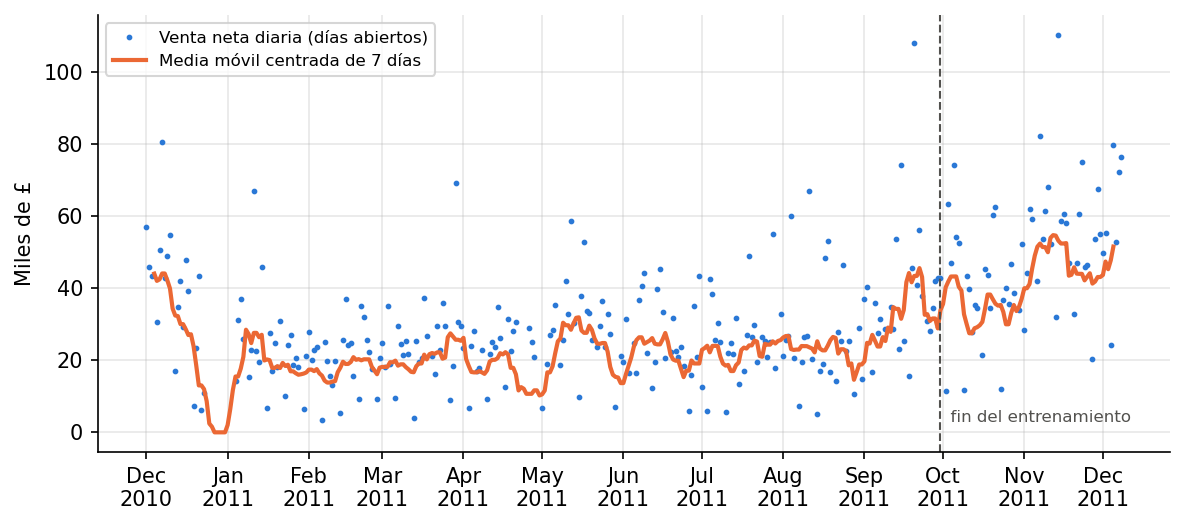
\includegraphics[width=\textwidth]{serie_diaria_media_movil.png}
\caption{Venta neta diaria de los días abiertos (puntos) y media móvil centrada de 7 días
calculada sobre el calendario completo con los días cerrados en cero (línea).}
\label{fig:serie}
\end{figure}

7 y no 5 ni 30 porque el ciclo de la serie es semanal: una ventana de siete días
calendario contiene exactamente un día de cada tipo (cinco días de semana, un sábado cerrado y
un domingo flojo), así que el patrón semanal se cancela y queda solo el nivel. Una ventana de 5
contiene a veces el sábado y el domingo y a veces ninguno, y la media oscila con el ciclo
semanal. Una de 30 no es múltiplo de 7, así que según dónde caiga cuenta cuatro o cinco
domingos, y además aplana cambios reales como el cierre de Navidad o la subida de septiembre.
Centrada para que $MA_t$ hable del día $t$. Una media de los siete días anteriores
describe el nivel de hace tres días y llega tarde a cualquier cambio de tendencia. La media
centrada no tiene ese retraso.

La serie empieza alta en diciembre de 2010 (unas \textsterling{}40\,000 diarias), cae a cero con el cierre de
fin de año y pasa enero a agosto casi plana, mayormente entre \textsterling{}15\,000 y \textsterling{}30\,000 de media
móvil, con caídas puntuales en las semanas de feriados (Semana Santa, la boda real y los feriados
de mayo) y una subida leve desde mayo. En septiembre arranca una subida fuerte que lleva el nivel a unas
\textsterling{}47\,000 en noviembre y diciembre, el doble que en verano. Es la temporada navideña de una
tienda que vende regalos a mayoristas, y diciembre de 2010 sugiere que el mismo pico ocurrió el
año anterior.

\subsection*{Inciso 3.2: estacionalidad}

\begin{table}[H]
\centering
\caption{Índice estacional de cada día abierto: promedio de $y_t/MA_t$ sobre los días abiertos
del entrenamiento.}\label{tab:indice}
\begin{tabular}{|c|c|c|c|c|c|c|}
\hline
Lunes & Martes & Miércoles & Jueves & Viernes & Domingo & Promedio \\
\hline
1.164 & 1.545 & 1.232 & 1.563 & 1.118 & 0.580 & 1.200 \\
\hline
\end{tabular}
\end{table}

\begin{figure}[H]
\centering
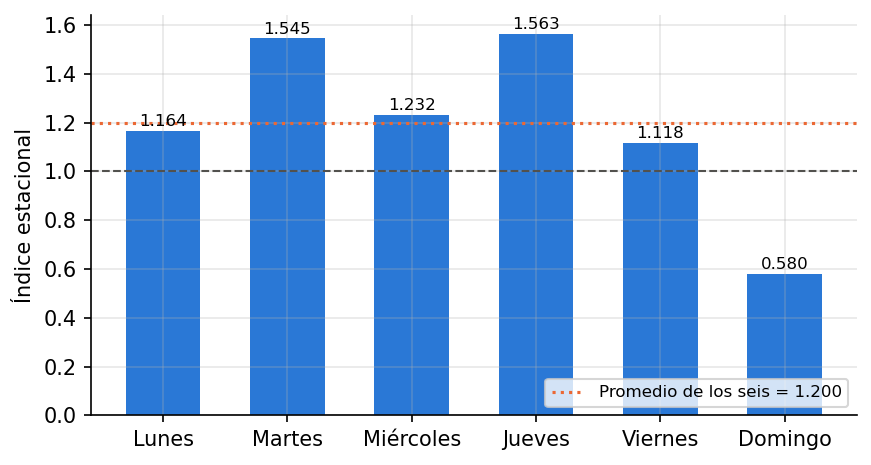
\includegraphics[width=0.7\textwidth]{indice_estacional.png}
\caption{Índice estacional por día de la semana. La línea gris marca 1 y la punteada el promedio
de los seis índices.}
\label{fig:indice}
\end{figure}

Martes y jueves son los días fuertes, con un 55\,\% más que la media móvil. Lunes, miércoles y
viernes quedan en torno a 1.2, y el domingo vende poco más de la mitad. El promedio de los
seis índices es 1.200 y no 1 porque la media móvil reparte la venta de la semana entre siete
días, sábado incluido, y el sábado siempre vale cero. Toda la venta de la semana la hacen los
seis días abiertos, así que en promedio cada uno queda $7/6\approx1.167$ veces arriba de la media
móvil. El 1.200 pasa de 1.167 por dos razones. Las semanas con feriado tienen solo cinco días
abiertos y su cociente se acerca a $7/5$, y el promedio de cocientes no es el cociente de los
promedios.

\subsection*{Inciso 3.3: autocorrelación}

\begin{figure}[H]
\centering
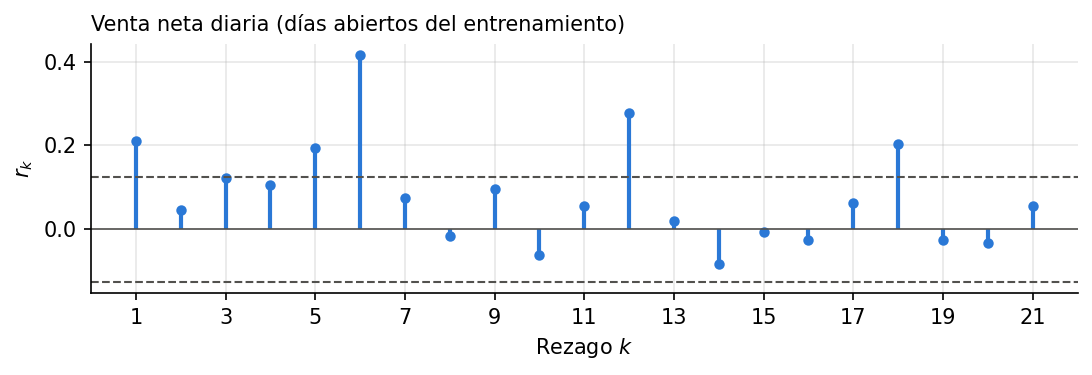
\includegraphics[width=0.9\textwidth]{acf_venta_entrenamiento.png}
\caption{ACF de la venta neta diaria sobre los 245 días abiertos del entrenamiento, una fila por
día, con las bandas $\pm1.96/\sqrt{245}=\pm0.125$.}
\label{fig:acf-venta}
\end{figure}

(a) De los 21 rezagos se salen 5: el 1, 5, 6, 12 y 18. Con $r_1=0.210$ la serie
reprueba la prueba de retardo 1 de la Tarea 2, que rechaza con $|r_1|>0.125$. El pico
está en el rezago 6 ($r_6=0.416$), y como no hay sábados, seis filas atrás es el mismo día de la
semana anterior, es decir, siete días calendario. Los rezagos 12 y 18 son las semanas 2 y
3. En las semanas con feriado hay solo cinco días abiertos, y ahí el mismo día de la semana
anterior queda cinco filas atrás; eso ayuda a explicar que el rezago 5 también se salga. La Ljung--Box no deja duda: $Q(6)=71.4$ con $p=2\times10^{-13}$ y $Q(12)=96.9$ con
$p=2\times10^{-15}$. Los dos valores de $m$ corresponden a los dos libros: $\log 245=5.5\approx6$
es el de Tsay y $2s=12$ con $s=6$ es el de FPP2, y aquí los dos cubren el periodo de 6 filas.

(b) Con lo de la Parte 0 se pueden separar dos cosas. Los picos en 6, 12 y 18 son el
patrón semanal, la misma huella que el proceso (b) de 0.4, y son media no constante, no memoria.
Lo que queda por debajo, una autocorrelación positiva en casi todos los rezagos cortos que baja
despacio, se parece a la tendencia del proceso (a), que es el nivel que sube en septiembre y el
salto de diciembre. Puede haber algo de memoria verdadera mezclada, pero con esta gráfica no se
puede separar. La Parte 4 quita primero lo que es media y después mira qué queda.

\section*{Parte 4: del AR(1) al SARIMA}

\subsection*{Incisos 4.1 y 4.2: quitar el día de la semana y probar un AR(1)}

La regresión contra las seis indicadoras, sin intercepto, estima la media de cada día: lunes
\textsterling{}26\,920, martes \textsterling{}34\,990, miércoles \textsterling{}27\,697, jueves \textsterling{}35\,270, viernes \textsterling{}26\,211 y domingo
\textsterling{}13\,706. Sus residuos $e_t$ son la venta menos la media de su día.

\begin{figure}[H]
\centering
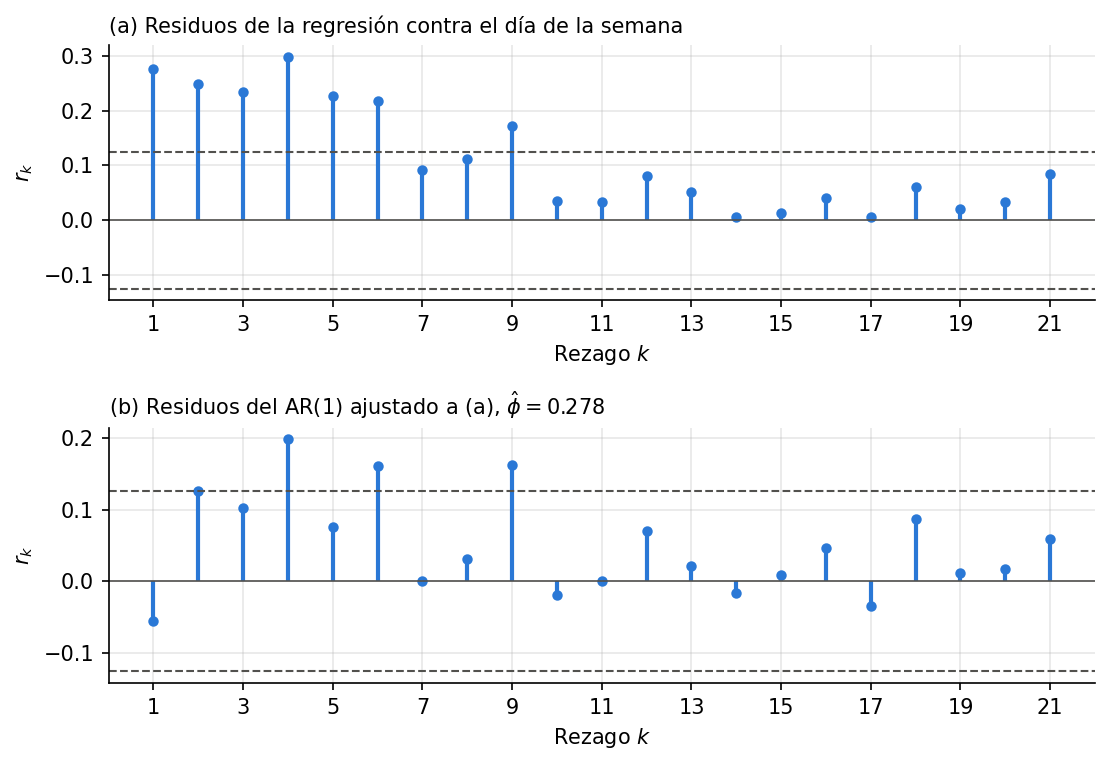
\includegraphics[width=0.9\textwidth]{acf_residuos_dia_semana_ar1.png}
\caption{(a) ACF de los residuos de la regresión contra el día de la semana. (b) ACF de los
residuos $u_t$ del AR(1) ajustado a esos residuos. Bandas $\pm1.96/\sqrt n$.}
\label{fig:acf-residuos}
\end{figure}

4.1. Los picos de 6, 12 y 18 desaparecieron, así que el patrón semanal sí era media
no constante y las indicadoras lo absorben. Pero ahora se salen los rezagos 1 a 6 y el 9, todos
entre 0.17 y 0.30, y la Ljung--Box empeora ($Q(6)=95.2$, $Q(12)=110.3$, $p<10^{-17}$). La forma
no es la de un AR(1). Con $r_1=0.28$ un AR(1) daría $r_2=0.08$ y $r_4=0.006$, y aquí $r_4$ vale
0.30. Se parece a la ACF de la tendencia de la figura~\ref{fig:acf-simulados}: valores parecidos
en muchos rezagos seguidos que bajan muy despacio. Al modelo le falta el nivel. Las
indicadoras suponen que un martes de febrero y uno de noviembre esperan lo mismo, y la
figura~\ref{fig:serie} muestra que no, así que los días de diciembre de 2010 y de
septiembre quedan con residuo positivo y los de enero a agosto con residuo negativo.

4.2. El AR(1) por OLS sobre $e_t$ da $\hat\phi=0.278$ (y $\hat c=-101.75$, prácticamente
cero, como debe ser con residuos de media cero). Sus residuos $u_t$ ya no tienen autocorrelación
en el rezago 1 ($r_1=-0.056$), pero siguen fuera de las bandas los rezagos 2, 4, 6 y 9, con
$r_4=0.198$. La Ljung--Box lo confirma con un grado de libertad menos: $Q(6)=25.1$ con 5 grados y
$p=1.4\times10^{-4}$, y $Q(12)=33.4$ con 11 grados y $p=4.5\times10^{-4}$. No alcanzó. Un
AR(1) con $\phi=0.28$ olvida en dos o tres días y no puede reproducir un nivel que cambia a lo
largo de meses. Para eso haría falta un $\phi$ cercano a 1, o directamente diferenciar. El rezago
6 que reaparece indica además que el efecto del día de la semana no es aditivo. Un martes de
septiembre vende más por encima de su media que un martes de febrero, porque la estacionalidad
crece con el nivel (es multiplicativa, como la descomposición de la Parte 3).

\subsection*{Inciso 4.3: SARIMA}

Se usa $s=6$ y no 7 porque el modelo trabaja con una fila por día abierto, y una semana
tiene seis días abiertos, así que el mismo día de la semana anterior está seis filas atrás. Un
$s=7$ compararía el lunes con el domingo de la semana anterior. La suposición se rompe cada vez
que entre dos filas hay un día de semana cerrado: en el cierre de Navidad, en Semana Santa, el día
de la boda real y en los lunes feriados de mayo y agosto. Entonces seis filas atrás ya no es el
mismo día de la semana. En el entrenamiento pasa en 28 de las 239 filas que tienen rezago 6, un
12\,\%.

Se usa el logaritmo porque la variación crece con el nivel. En noviembre las diferencias
entre días son de decenas de miles de libras, y en febrero de unos pocos miles. Es el caso en que
FPP2 recomienda transformar. El logaritmo además convierte la estacionalidad multiplicativa en
aditiva ($\log(T\cdot S\cdot R)=\log T+\log S+\log R$), y al volver con $\exp$ el pronóstico
siempre sale positivo. Se puede aplicar porque el día con menos venta tiene \textsterling{}3\,440 y ningún día
abierto tiene venta neta cero o negativa.

\begin{table}[H]
\centering
\caption{Ajuste de S1 y S2 sobre el logaritmo de la venta de los 245 días abiertos del
entrenamiento, con el límite de iteraciones por defecto (50) y con 500.}\label{tab:sarima}
\small
\begin{tabular}{|c|c|c|c|c|p{5.6cm}|}
\hline
Modelo & \texttt{maxiter} & Convergió & Iteraciones & Log-verosimilitud & Parámetros \\
\hline
S1 & 50 & No & 50 & -185.20 & \texttt{intercept = 0.9016, ar.L1 = 0.1870, ar.S.L6 = 0.8883, sigma2 = 0.2863} \\
S1 & 500 & Sí & 80 & -160.70 & \texttt{intercept = 4.2117, ar.L1 = 0.1319, ar.S.L6 = 0.5207, sigma2 = 0.2157} \\
S2 & 50 & Sí & 14 & -156.94 & \texttt{ma.L1 = -0.9142, ma.S.L6 = -0.6698, sigma2 = 0.2131} \\
S2 & 500 & Sí & 14 & -156.94 & \texttt{ma.L1 = -0.9142, ma.S.L6 = -0.6698, sigma2 = 0.2131} \\
\hline
\end{tabular}
\end{table}

S1 no converge con el límite por defecto. El optimizador se detiene en 50 iteraciones y
los parámetros que devuelve están lejos del óptimo. Con 500 converge en 80 iteraciones, la
log-verosimilitud mejora en 24.5 puntos y los parámetros cambian mucho: el AR estacional baja de
0.888 a 0.521 y la varianza del error de 0.286 a 0.216. El modelo sin converger sobreestimaba la
persistencia semanal, y si no se revisa \texttt{mle\_retvals} no hay ningún aviso de que esos
números están mal. S2 converge en 14 iteraciones y no cambia al subir el límite. En todo
lo que sigue S1 se ajusta con \texttt{maxiter=500}. Los parámetros de S2 dicen algo del nivel:
$\theta=-0.914$ está cerca de $-1$, y entonces el factor $(1+\theta B)$ casi cancela la diferencia
$(1-B)$. Es la forma ARIMA del suavizamiento exponencial, con peso $1+\theta=0.086$ para cada dato
nuevo, así que el nivel que sigue S2 se mueve despacio: casi no reacciona a un día suelto
y solo se ajusta cuando el cambio dura varias semanas.

\subsection*{Inciso 4.4: diagnóstico}

\begin{figure}[H]
\centering
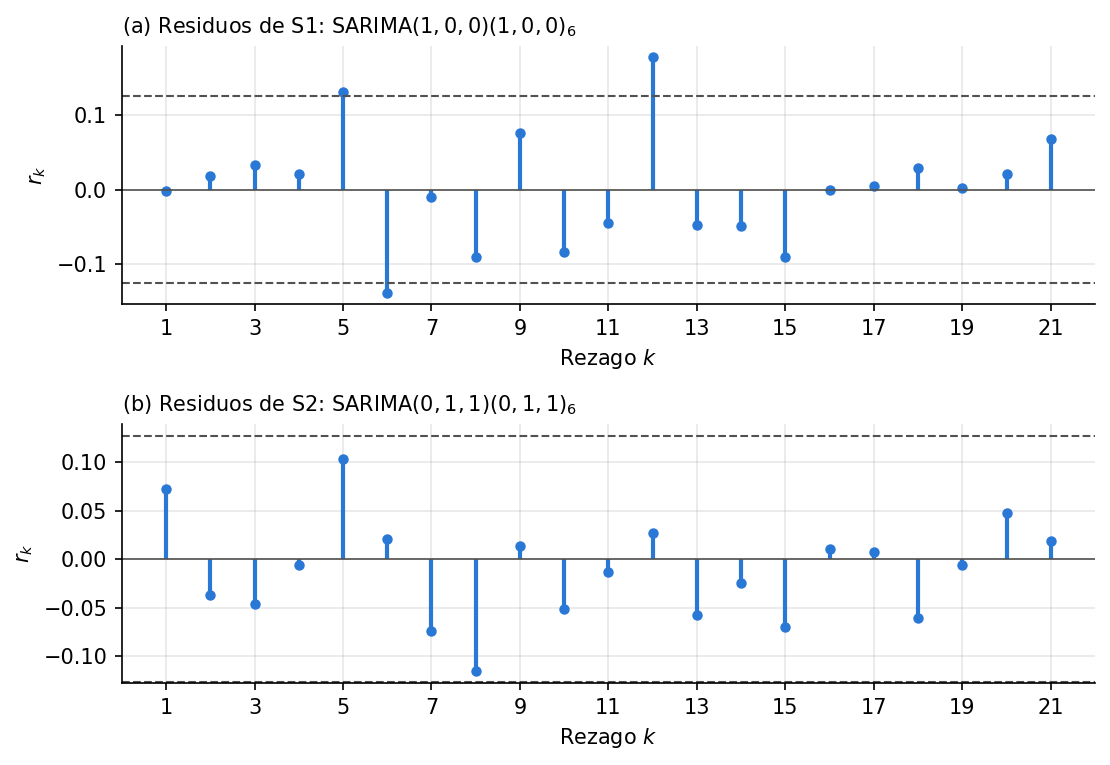
\includegraphics[width=0.9\textwidth]{acf_residuos_sarima.png}
\caption{ACF de los residuos de S1 (245 residuos) y de S2 (sin los 7 primeros, 238 residuos), con
bandas $\pm1.96/\sqrt n$.}
\label{fig:acf-sarima}
\end{figure}

Con $m-2$ grados de libertad (dos coeficientes ARMA estimados en cada modelo):

\begin{table}[H]
\centering
\caption{Ljung--Box sobre los residuos de los dos SARIMA.}\label{tab:diagnostico}
\begin{tabular}{|l|c|c|c|c|}
\hline
Modelo & $Q(6)$ & $p$ (4 g.l.) & $Q(12)$ & $p$ (10 g.l.) \\
\hline
S1 & 9.57 & 0.048 & 23.54 & 0.009 \\
S2 & 4.88 & 0.300 & 10.49 & 0.398 \\
\hline
\end{tabular}
\end{table}

S2 deja residuos de ruido blanco. Ninguno de sus 21 rezagos sale de las bandas, y la
Ljung--Box no rechaza con ninguno de los dos $m$. S1 no. Rechaza con $m=12$ al 1\,\% y con $m=6$
apenas al 5\,\%, y le quedan fuera los rezagos 5, 6 y 12. Es el mismo problema de 4.1 y 4.2: un
modelo estacionario supone una media fija, y la media de esta serie se mueve. El AR estacional
de S1 copia parte del patrón semanal, pero no puede seguir un nivel que cambia. La doble
diferencia de S2 trabaja con cambios y no con niveles, y ahí la media que se mueve deja de ser un
problema.

\subsection*{Inciso 4.5: hacia dónde van los pronósticos}

\begin{figure}[H]
\centering
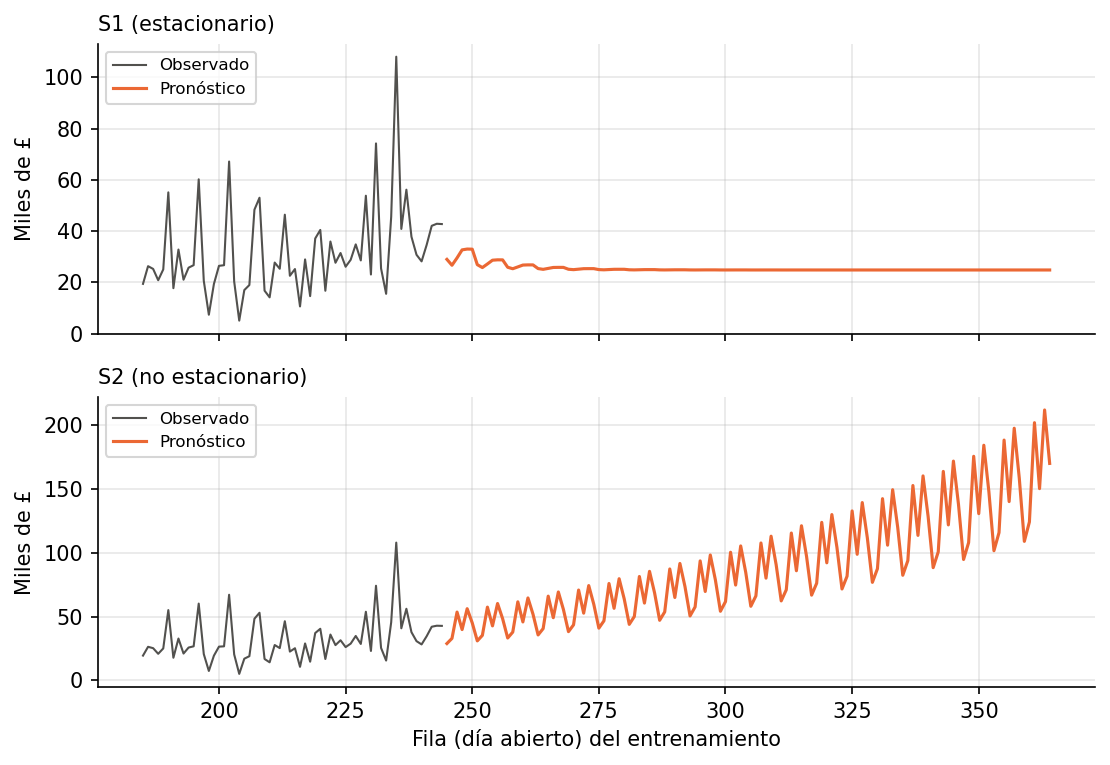
\includegraphics[width=0.9\textwidth]{pronostico_largo_s1_s2.png}
\caption{Pronóstico a 120 días abiertos desde el final del entrenamiento, ya en libras, con los
últimos 60 días observados en gris.}
\label{fig:pronostico-largo}
\end{figure}

S1 es estacionario, como el AR(1) con $|\phi|<1$, así que su pronóstico vuelve a la
media. En el AR(1) el pronóstico a $h$ pasos es $\mu+\phi^h(y_n-\mu)$, y $\phi^h\to0$. Para S1 la
media en logaritmo es $c/((1-\phi)(1-\Phi))=4.2117/(0.8681\cdot0.4793)=10.12$, que en libras es
\textsterling{}24\,878, casi la media geométrica del entrenamiento (\textsterling{}24\,156). En la figura el pronóstico sale
de los últimos valores, conserva unas semanas el patrón semanal (que se apaga como
$\Phi^{h/6}$) y a las cinco o seis semanas ya es una línea plana en \textsterling{}24\,878, haya pasado lo que haya pasado
en septiembre.

S2 no es estacionario, como la caminata aleatoria, así que no vuelve a ninguna media. Su
pronóstico arrastra el último nivel y el último patrón semanal, y además una pendiente.
$(1-B)(1-B^6)=(1-B)^2(1+B+\dots+B^5)$ tiene una raíz unitaria doble, y la parte de largo plazo de
su pronóstico es un nivel más una recta más un patrón semanal que se repite. La recta sale de
la subida de septiembre y, como está en logaritmo, en libras es crecimiento exponencial: a los
120 días abiertos pronostica entre \textsterling{}109\,000 y \textsterling{}212\,000 diarios. Igual que la varianza de la
caminata crece como $t\sigma^2$, la incertidumbre de S2 crece sin límite con el horizonte. A una
semana, la cualidad que lo hace absurdo a cuatro meses (seguir el nivel más reciente en lugar de
volver al promedio del año) es justo lo que hace falta, como muestra la Parte 5.

\section*{Parte 5: pronóstico y fuga}

\subsection*{Inciso 5.1: los modelos}

Los seis modelos están en \texttt{modelos\_pronostico.py}. B1 es la media de todos los días
abiertos hasta el origen. B2 copia el valor del mismo día de la semana abierto más reciente. M1 es
OLS con las seis indicadoras y una tendencia lineal $t$ (días calendario desde el 1 de diciembre
de 2010). M2 es OLS con las seis indicadoras, $y_{t-7}$ y $y_{t-14}$. Si un rezago cae en día
cerrado se retrocede de siete en siete hasta un día abierto: para el lunes 9 de mayo los dos
rezagos son el 18 de abril, y el script lo verifica. Las filas sin rezago (las dos primeras
semanas de diciembre de 2010) no se usan para ajustar. S1 y S2 se reajustan en cada origen con
\texttt{maxiter=500}. En los 64 ajustes (22 orígenes de (b) y 10 de (c), por dos modelos)
\texttt{mle\_retvals['converged']} fue verdadero.

M2 puede usar $y_{t-7}$ para cualquiera de los siete días siguientes porque el objetivo
más lejano es el domingo siguiente, origen $+7$, y su $y_{t-7}$ es el propio domingo del origen,
que ya se observó. Todos los $y_{t-7}$ de la semana caen en la semana que ya pasó. No podría
usar $y_{t-1}$, porque para el martes $y_{t-1}$ es el lunes, que el domingo todavía no ha
ocurrido. Funcionaría solo para el primer día de la semana. S1 usa el rezago 1 de todas
formas pronosticando de forma recursiva. Para el segundo día usa en lugar de $y_{t-1}$ su propio
pronóstico del primero, y así sucesivamente. Es legítimo, porque solo usa información del origen,
pero los errores se acumulan con el horizonte.

\subsection*{Inciso 5.2: tres formas de estimar el error}

\begin{table}[H]
\centering
\caption{Error en libras de cada modelo. (a) Validación cruzada aleatoria de 5 folds sobre los 245
días del entrenamiento, media y desviación estándar (entre paréntesis) de 10 repeticiones. (b)
Origen móvil semanal con 22 orígenes, del domingo 1 de mayo al 25 de septiembre, 128 días
evaluados. (c) Periodo de prueba con origen móvil semanal, 10 orígenes del 2 de octubre al 4 de
diciembre, 58 días evaluados.}\label{tab:validacion}
\small
\begin{tabular}{|l|c|c|c|c|c|c|}
\hline
& \multicolumn{2}{c|}{(a) CV aleatoria} & \multicolumn{2}{c|}{(b) Origen móvil (entrenamiento)} & \multicolumn{2}{c|}{(c) Prueba} \\
\cline{2-3}\cline{4-5}\cline{6-7}
Modelo & MAE & RMSE & MAE & RMSE & MAE & RMSE \\
\hline
B1 & 10\,230 (25) & 14\,216 (33) & 10\,254 & 14\,936 & 22\,472 & 27\,061 \\
B2 & -- & -- & 11\,341 & 15\,652 & 14\,409 & 18\,637 \\
M1 & 9\,145 (138) & 12\,565 (154) & 9\,832 & 13\,901 & 15\,202 & 20\,283 \\
M2 & 8\,293 (121) & 11\,736 (159) & 9\,258 & 13\,413 & 15\,218 & 19\,917 \\
S1 & -- & -- & 9\,657 & 13\,767 & 16\,738 & 21\,052 \\
S2 & -- & -- & 10\,057 & 14\,027 & 12\,545 & 15\,901 \\
\hline
\end{tabular}
\end{table}

(a) no tiene sentido para B2, S1 y S2 porque esos modelos son la historia reciente
ordenada. B2 no se ajusta (copia el valor de la semana anterior), así que no hay nada que
entrenar en cuatro folds. Si se aplicara de todos modos, el ``mismo día más reciente'' podría
estar después del día que se predice. S1 y S2 son recursiones sobre filas consecutivas, y una
partición al azar deja huecos en la serie y pondría a predecir un día de mayo con un modelo que
ya vio junio. Eso es interpolar y no pronosticar. B1, M1 y M2 sí se pueden ajustar sobre filas
sueltas, porque sus predictores (indicadoras, $t$, rezagos ya calculados) están en cada fila.

(b) se acerca más a (c) que (a). Para los tres modelos que tienen las dos, (a) da el error
más bajo: el MAE de M2 es 8\,293 en (a), 9\,258 en (b) y 15\,218 en (c). Pero ninguna se
acerca de verdad. El error de prueba es entre un 25\,\% y un 120\,\% mayor que lo que estimaron, y además
las dos ordenan mal los modelos. Dentro del entrenamiento, el origen móvil pone a M2 primero, S1 segundo y
a B2 último, y en la prueba gana S2 y B2 queda segundo. Dentro del entrenamiento (con el nivel
casi plano de mayo a agosto) un modelo que se ajusta lento a los cambios no pierde nada. En la
prueba el nivel cambió, y eso cambió quién gana.

\subsection*{Inciso 5.3: quién gana en prueba y por qué}

\begin{figure}[H]
\centering
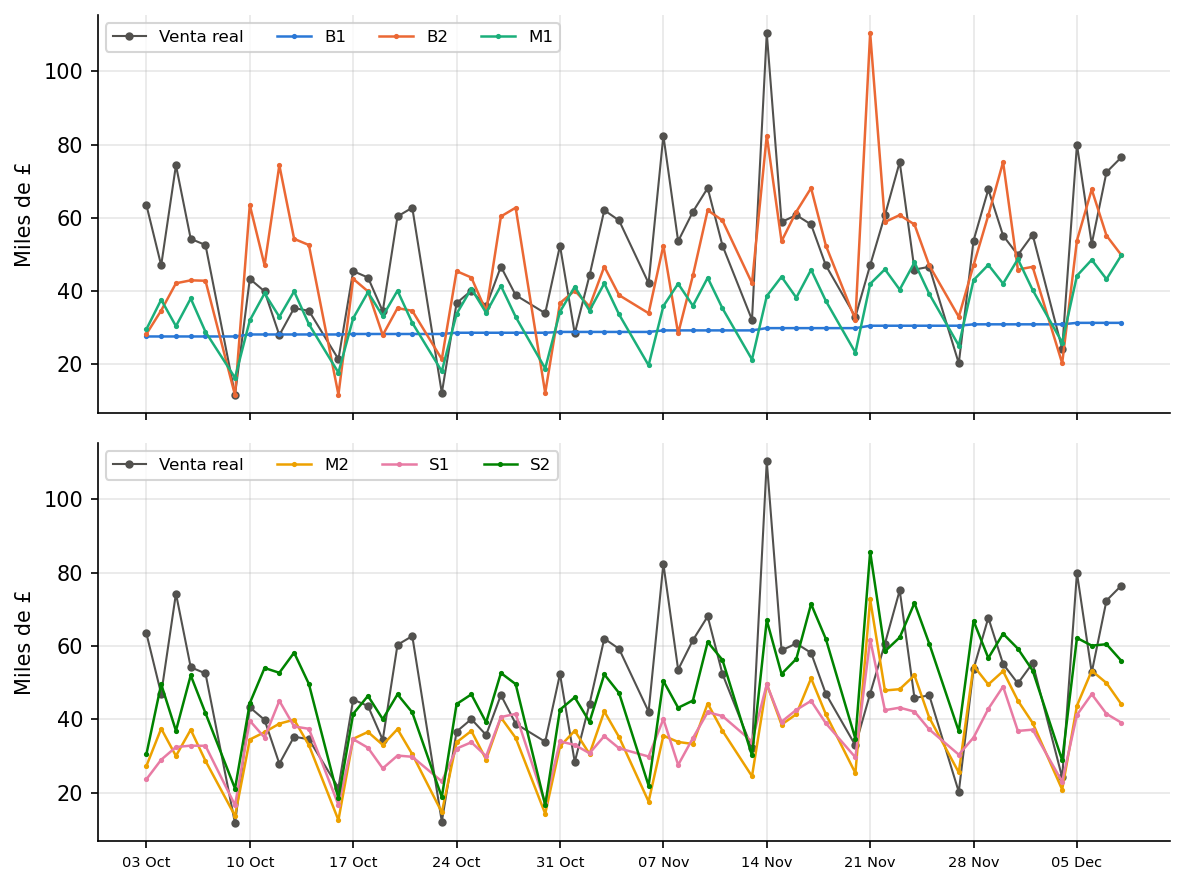
\includegraphics[width=\textwidth]{pronosticos_prueba.png}
\caption{Pronósticos del origen móvil semanal contra la venta real del 3 de octubre al 8 de
diciembre de 2011 (en gris). Arriba los tres modelos de referencia, abajo M2 y los dos SARIMA.}
\label{fig:pronosticos-prueba}
\end{figure}

Gana S2, con MAE de \textsterling{}12\,545 y RMSE de \textsterling{}15\,901, seguido de B2. Lo que los separa del resto
es el nivel. La venta media de los días abiertos del entrenamiento fue \textsterling{}27\,632 y la de la prueba
\textsterling{}49\,768, y de mes a mes pasó de \textsterling{}26\,800 en agosto a \textsterling{}38\,900 en septiembre, \textsterling{}40\,800 en
octubre, \textsterling{}54\,900 en noviembre y \textsterling{}58\,700 en diciembre. El sesgo medio en prueba (pronóstico menos
real) lo resume:

\begin{center}
\begin{tabular}{|l|c|c|c|c|c|c|}
\hline
& B1 & B2 & M1 & M2 & S1 & S2 \\
\hline
Sesgo medio (\textsterling{}) & $-20\,530$ & $-2\,743$ & $-13\,756$ & $-12\,902$ & $-14\,227$ & $-1\,187$ \\
\hline
\end{tabular}
\end{center}

B1, M1, M2 y S1 están anclados al pasado: B1 a la media del año, M1 a una recta ajustada sobre
un año casi plano, M2 a coeficientes que pesan poco los rezagos, y S1 tira hacia su media de largo plazo, que en
cada reajuste sigue muy por debajo del nivel de otoño. Los cuatro reaccionan tarde a la subida y
se quedan cortos por \textsterling{}13\,000 a \textsterling{}20\,000 diarios en promedio. En la figura~\ref{fig:pronosticos-prueba} se ve que las
líneas de abajo, salvo la verde, van casi siempre por debajo de la gris. S2 y B2 siguen el nivel
más reciente y no tienen ese sesgo. B2 lo sigue copiando, y por eso copia también los picos
sueltos: el lunes 14 de noviembre vendió \textsterling{}110\,000 y B2 pronosticó \textsterling{}110\,000 para el lunes 21. S2
lo sigue suavizando ($1+\theta=0.086$), con el patrón semanal aparte, y por eso tiene menos ruido
que B2.

La respuesta a 4.4 dice lo mismo desde los residuos. S2 era el único modelo que dejaba ruido
blanco, es decir, el único que había capturado toda la estructura de la serie, incluido el nivel
que se mueve. S1 dejaba autocorrelación en los rezagos 5, 6 y 12, y esa es información sobre el
futuro que el modelo no aprovecha. Cuando el nivel cambió en otoño, lo que S1 no había capturado
en el entrenamiento se convirtió en error de pronóstico.

\subsection*{Inciso 5.4: la trampa}

\begin{table}[H]
\centering
\caption{M2 con y sin la media móvil centrada de 7 días como predictor.}\label{tab:trampa}
\begin{tabular}{|l|c|c|c|c|}
\hline
& \multicolumn{2}{c|}{(a) CV aleatoria} & \multicolumn{2}{c|}{(b) Origen móvil} \\
\cline{2-3}\cline{4-5}
Modelo & MAE & RMSE & MAE & RMSE \\
\hline
M2 & 8\,293 (121) & 11\,736 (159) & 9\,258 & 13\,413 \\
M2 + media móvil & 7\,416 (78) & 10\,028 (96) & 8\,378 & 11\,363 \\
\hline
\end{tabular}
\end{table}

Se ve mejor: baja el MAE un 10\,\% con las dos validaciones y el RMSE un 15\,\%. Es una mejora
falsa. La media móvil centrada del día $t$ es el promedio de $y_{t-3},\dots,y_{t+3}$. Contiene la
propia venta que se quiere pronosticar y la de los tres días siguientes, así que es un
predictor ilegal: le pasa al modelo una séptima parte de la respuesta, más el nivel de
los días que vienen después.

El origen móvil no lo detecta porque la media móvil se calculó una sola vez sobre toda la serie y
quedó guardada como una columna más. El origen móvil controla qué filas se usan para
ajustar y cuáles para evaluar, pero no qué información trae cada predictor. Si la columna ya
tiene el futuro adentro, cortar las filas en el origen no la limpia. La fuga está en cómo se
construyó la variable, no en cómo se partieron los datos.

Y (c) no se puede calcular sin hacer trampa. El domingo del origen, la media móvil del
lunes siguiente necesita las ventas de viernes a jueves, y cuatro de esas (lunes a jueves) aún no
han ocurrido. Para el 6, 7 y 8 de diciembre ni siquiera existe, porque necesita días posteriores al
final de los datos. Haciendo la trampa, en los 55 días de prueba donde existe, M2 con la media
móvil tendría un MAE de \textsterling{}9\,113 contra \textsterling{}15\,043 del M2 honesto. Es el mejor número de todo el
trabajo, y no se puede reproducir en la vida real.

\subsection*{Inciso 5.5: por qué todo se queda corto}

Hay dos causas. La primera viene de cómo se partieron los datos. La validación cruzada
aleatoria pone en el entrenamiento los días vecinos del día evaluado, antes y después. Con una
serie autocorrelacionada eso es interpolar: el martes se adivina mejor si se conoce el lunes y el
miércoles. Por eso (a) da siempre el error más bajo. Esta causa se arregla con una mejor
validación, respetando el tiempo como hace el origen móvil, y por eso (b) se acerca más a (c).

La segunda es que la serie cambió. La prueba cae en la temporada navideña, con un nivel
1.8 veces el del entrenamiento, y ninguna partición del entrenamiento contiene un periodo así.
Enero a septiembre no tienen un otoño del cual aprender. Esta causa no se arregla validando
mejor, porque ninguna validación hecha con datos de un régimen puede medir el error en un régimen
que nunca vio. Solo se arregla con datos que contengan ese régimen, es decir, con el otoño de
otros años.

Con un solo año no se puede estimar la estacionalidad anual. Para separar un efecto
estacional de una tendencia hace falta ver el ciclo al menos dos veces. Aquí cada mes aparece una
sola vez, y la subida de septiembre a diciembre de 2011 podría ser temporada navideña, crecimiento
del negocio o las dos cosas. Diciembre de 2010, que también fue alto (\textsterling{}37\,900 diarios), sugiere que
es temporada, pero es un solo dato. Por eso, y por la regla de FPP2 de tener al menos dos periodos
completos, los modelos de esta tarea solo tienen estacionalidad semanal.

\section*{Parte 6: detrás de la serie hay clientes: análisis RFM}

\subsection*{Inciso 6.1: R, F y M al 1 de octubre}

Con los datos limpios que tienen \texttt{CustomerID} y solo las transacciones anteriores al 1 de
octubre de 2011, hay 3\,615 clientes con al menos una factura de venta. La recencia es el
número de días entre la fecha de su última factura de venta y el 1 de octubre (1 para quien
compró el 30 de septiembre). La frecuencia es el número de facturas de venta distintas, sin
contar las cancelaciones, y el monto es la venta neta, con las cancelaciones restando. Otros 43
clientes solo tienen cancelaciones antes del corte (devoluciones de pedidos anteriores a diciembre
de 2010), no tienen ninguna compra que dé recencia o frecuencia, y no entran.

13 clientes tienen $M\le0$: 6 con monto exactamente cero y 7 negativo, que suman
$-$\textsterling{}1\,981. Son clientes que devolvieron todo lo que compraron o más, porque devolvieron
mercancía comprada antes de que empezaran los datos. Entre ellos está el 12346 del inciso 1.4, con
$F=1$ y $M=0$. Se quedan en el análisis, porque 6.2 los incluye en el orden, y caen en el
puntaje de monto más bajo, que es lo que les corresponde porque no han dejado ingreso. Lo que no
se hace es interpretar su $M$ como un monto de compra.

No se puede usar nada posterior al 1 de octubre porque en 6.3 la variable que se quiere predecir
es si el cliente compró después de esa fecha. Si una compra de noviembre entrara en la recencia,
el cliente aparecería como reciente justo porque compró. Sería el predictor ilegal de 5.4 otra
vez, con la respuesta metida en el predictor, y el AUC saldría inflado.

\subsection*{Inciso 6.2: puntajes por quintiles}

El problema con F es que hay demasiados empates. El 40.1\,\% de los clientes tiene $F=1$ y el
19.1\,\% $F=2$, así que los cuantiles del 20\,\% y del 40\,\% valen los dos 1, y
\texttt{pd.qcut(F, 5)} falla con ``Bin edges must be unique''. No hay forma de partir en cinco
grupos de igual tamaño a clientes que tienen exactamente el mismo valor.

Con el desempate del enunciado (orden por \texttt{CustomerID}, permutación con
\texttt{default\_rng(2026)} y \texttt{qcut} sobre \texttt{rank(method='first')}) cada puntaje
queda con 723 clientes. Los 1\,449 clientes con $F=1$ se reparten en 723 con puntaje 1, 723 con
puntaje 2 y 3 con puntaje 3. El mismo procedimiento se aplicó a R y a M para que las tres
dimensiones tengan puntajes reproducibles. Lo que esto implica es que dos clientes con la misma
$F$ pueden tener puntajes distintos por sorteo, y esa diferencia no dice nada del cliente. Con
otra semilla se intercambian. La tabla~\ref{tab:tasa-compra} lo confirma: los puntajes 1 y 2 de
frecuencia, que son todos clientes con $F=1$, compran en proporciones casi iguales (0.329 y
0.310), y el 2 hasta queda un poco por debajo.

\subsection*{Inciso 6.3: \textquestiondown{}quién vuelve a comprar?}

De los 3\,615 clientes, 1\,835 (el 50.8\,\%) hicieron al menos una compra entre el 1 de octubre y el 8
de diciembre.

\begin{table}[H]
\centering
\caption{Fracción de clientes que compró entre el 1 de octubre y el 8 de diciembre, por puntaje
(5 es el mejor).}\label{tab:tasa-compra}
\begin{tabular}{|l|c|c|c|c|c|c|}
\hline
Puntaje & 1 & 2 & 3 & 4 & 5 & 5 menos 1 \\
\hline
Recencia & 0.277 & 0.385 & 0.550 & 0.664 & 0.663 & 0.386 \\
Frecuencia & 0.329 & 0.310 & 0.450 & 0.593 & 0.856 & 0.527 \\
Monto & 0.295 & 0.373 & 0.455 & 0.610 & 0.805 & 0.510 \\
\hline
\end{tabular}
\end{table}

\begin{figure}[H]
\centering
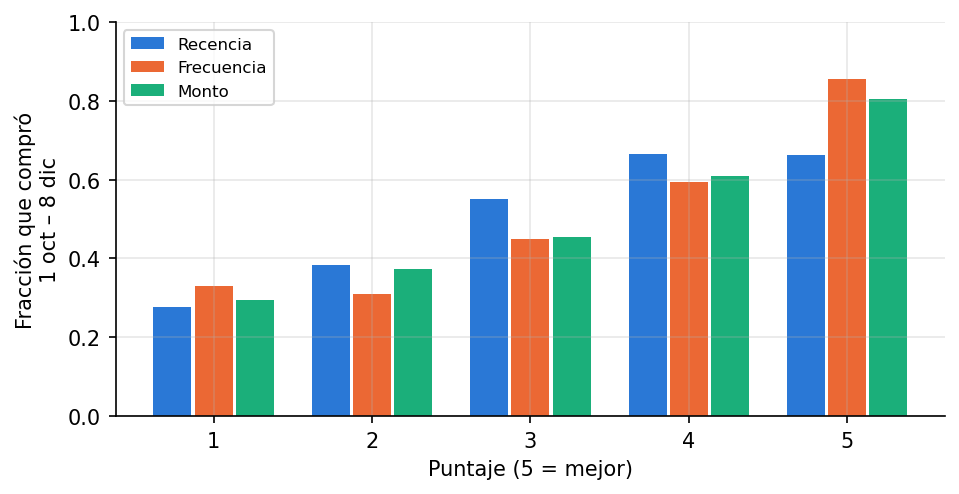
\includegraphics[width=0.75\textwidth]{rfm_tasa_compra_por_puntaje.png}
\caption{La misma información de la tabla~\ref{tab:tasa-compra}.}
\label{fig:rfm}
\end{figure}

\begin{table}[H]
\centering
\caption{AUC de cada dimensión como clasificador de $\text{compra}_i$. El AUC es la probabilidad
de que un comprador tenga un valor más alto que un no comprador, y se calcula con la fórmula de
Mann--Whitney a partir de los rangos.}\label{tab:auc}
\begin{tabular}{|l|c|}
\hline
Variable & AUC \\
\hline
Recencia ($-R$, crudo) & 0.6720 \\
Frecuencia ($F$, crudo) & 0.7201 \\
Monto ($M$, crudo) & 0.7086 \\
Suma de los tres puntajes & 0.7338 \\
\hline
\end{tabular}
\end{table}

La frecuencia es la que mejor separa. Su puntaje 5 compra en un 86\,\%, casi tres veces que
el puntaje 1, y tiene el AUC individual más alto (0.720). El monto está cerca (0.709), y tiene
sentido, porque quien compra muchas veces suele acumular mucho monto. La recencia es la más débil
(0.672) y se aplana arriba: los puntajes 4 y 5 compran igual (0.664 y 0.663). Con un periodo de
compra de diez semanas, haber comprado hace 10 días o hace 30 da lo mismo. Lo que separa es
haber comprado en los últimos meses o no. La suma de los tres puntajes da el mejor AUC (0.734),
aunque solo un poco más que F sola, porque las tres dimensiones repiten buena parte de la misma
información.

\subsection*{Incisos 6.4 y 6.5: campeones y clientes nuevos}

\begin{table}[H]
\centering
\caption{Reparto de la venta neta del 1 de octubre al 8 de diciembre entre todos los clientes
con \texttt{CustomerID}, incluidos los nuevos.}\label{tab:reparto}
\resizebox{\textwidth}{!}{
\begin{tabular}{|l|c|c|c|c|}
\hline
Grupo & N.º de clientes & Fracción de clientes & Venta oct--dic (\textsterling{}) & Fracción de la venta \\
\hline
Campeones (4 o 5 en R, F y M) & 777 & 0.215 & 1\,278\,410 & 0.533 \\
Resto de clientes con historia & 2838 & 0.785 & 744\,419 & 0.310 \\
Clientes nuevos & 723 & -- & 377\,860 & 0.157 \\
\hline
Total con \texttt{CustomerID} & & & 2\,400\,689 & 1.000 \\
\hline
\end{tabular}}
\end{table}

6.4. Los campeones son 777 clientes, el 21.5\,\% de los clientes de 6.1, y
generaron el 53.3\,\% de la venta neta de octubre a diciembre de todos los clientes con
\texttt{CustomerID}. El 81.6\,\% de ellos volvió a comprar. Es la regla de Pareto que justifica
el RFM: una quinta parte de los clientes sostiene la mitad de la venta.

6.5. Los clientes nuevos, que no tienen ninguna factura de venta antes del 1 de
octubre, son 723 y generaron el 15.7\,\% de esa venta, \textsterling{}377\,860. Ningún análisis
RFM ni ningún modelo cliente por cliente puede pronosticar esa venta, porque esos clientes no
existen en la tabla del 1 de octubre. No tienen R, F ni M, y no hay ninguna fila a la que asignarles
una probabilidad de compra. Un pronóstico bottom-up, que pronostica cada cliente conocido y
suma, deja fuera por construcción ese 15.7\,\%. Si además se arma solo con clientes identificados,
deja fuera también la venta sin \texttt{CustomerID}, que en el mismo periodo es el 17.2\,\% del
total (\textsterling{}497\,371 de \textsterling{}2\,898\,060). Para la venta total, los nuevos son el 13.0\,\%.

El pronóstico de la Parte 5 es top-down: pronostica el total, y el total ya incluye cada día
la venta de los clientes que llegaron por primera vez, con o sin \texttt{CustomerID}. No sabe
quiénes son, pero sí sabe cuánto suelen aportar en conjunto, porque eso está en la historia de la
serie. Por eso el top-down puede ver a los clientes nuevos y el bottom-up no. Para el
proyecto del curso, que compara los dos enfoques, el bottom-up tendrá un sesgo hacia abajo de al
menos la venta de los clientes que todavía no existen, y en una tienda que crece en otoño ese
sesgo crece justo cuando más importa, igual que el sesgo de los modelos anclados al pasado en la
Parte 5. La única forma de corregirlo es agregarle al bottom-up un modelo aparte para la llegada de
clientes nuevos, que es un pronóstico agregado.

\section*{Referencias}

\begin{itemize}
\item D.~Chen. Online Retail [conjunto de datos]. UCI Machine Learning Repository, 2015. \url{https://archive.ics.uci.edu/dataset/352/online+retail}

\item D.~Chen, S.~L.~Sain y K.~Guo. ``Data mining for the online retail industry: A case study of RFM model-based customer segmentation using data mining''. Journal of Database Marketing \& Customer Strategy Management 19.3, 2012, pp.~197--208.

\item R.~J.~Hyndman y G.~Athanasopoulos. Forecasting: Principles and Practice. 2.\textsuperscript{a} ed. OTexts, Melbourne, 2018. \url{https://otexts.com/fpp2/}. Capítulos 2, 3, 6, 8, 10 y 12.

\item R.~S.~Tsay. Analysis of Financial Time Series. 2.\textsuperscript{a} ed. Wiley, 2005. Capítulo 2, secciones 2.1 a 2.8.

\item G.~E.~P.~Box, G.~M.~Jenkins, G.~C.~Reinsel y G.~M.~Ljung. Time Series Analysis: Forecasting and Control. 5.\textsuperscript{a} ed. Wiley, 2015. Capítulo 9 (el modelo de aerolínea).

\item G.~M.~Ljung y G.~E.~P.~Box. ``On a measure of lack of fit in time series models''. Biometrika 65.2, 1978, pp.~297--303.

\item F.~H.~C.~Marriott y J.~A.~Pope. ``Bias in the estimation of autocorrelations''. Biometrika 41.3/4, 1954, pp.~390--402.

\item GOV.UK. UK bank holidays. \url{https://www.gov.uk/bank-holidays}

\item S.~Seabold y J.~Perktold. ``Statsmodels: Econometric and statistical modeling with Python''. Proceedings of the 9th Python in Science Conference, 2010.
\end{itemize}

\end{document}
